\documentclass[11pt,letterpaper]{article}
\usepackage[T1]{fontenc}
\usepackage{lmodern,microtype}
\usepackage[margin=0.88in,headheight=14pt]{geometry}
\usepackage{amsmath,amssymb,amsthm,booktabs,fancyhdr,xcolor,tikz}
\usepackage[colorlinks=true,linkcolor=black,urlcolor=blue!55!black,citecolor=black]{hyperref}
\hypersetup{pdftitle={Counting the first corona of a rhombus},pdfauthor={Blake Stone, with OpenAI Codex}}
\pagestyle{fancy}\fancyhf{}\lhead{\small Counting the first corona of a rhombus}\rhead{\small Blake Stone}\cfoot{\thepage}
\newtheorem{theorem}{Theorem}[section]
\newtheorem{lemma}[theorem]{Lemma}
\newcommand{\one}{\mathbf 1}
\newcommand{\floor}[1]{\left\lfloor #1\right\rfloor}
\newcommand{\oid}[1]{\href{https://oeis.org/A#1}{A#1}}
\newcommand{\cc}[2]{\binom{#1}{#2}}
\setlength{\parskip}{0.16em}
\raggedbottom
\begin{document}
\thispagestyle{plain}
\begin{center}
{\LARGE\bfseries Counting the first corona of a rhombus\par}
\vspace{0.35em}
{\large Closed formulas, column recurrences and symmetry classes\par}
\vspace{0.7em}
Blake Stone\\
{\small Research manuscript prepared with OpenAI Codex}
\end{center}
\begin{abstract}
L. Edson Jeffery gave a finite construction for the first ring of rhombi around a fixed central tile. He asked whether any column of the resulting table satisfies a recurrence. We give a closed expression for every entry and show that each column has least constant-coefficient recurrence order 13. The expression proves his row congruence modulo $2^{n-3}$ and determines when the modulus is sharp in the first column. Up to isometry, the least eventual order is 20. For a $45^\circ$ central rhombus the symmetry count is 385, a correction to the value 414 in \oid{233333}. We also prove the proposed recurrences and generating functions for the four edge-neighbor tiles.
\end{abstract}

\section{Jeffery's first-corona problem}
Fix $n\ge2$ and $1\le k\le\floor{n/2}$. All tiles have unit edge length and angles that are positive multiples of $\pi/n$. The distinguished central tile has angles $k\pi/n$ and $(n-k)\pi/n$. Its \emph{first corona} includes the center and its edge- and vertex-neighbors. The center together with just its four edge-neighbors is a \emph{core}. We enumerate the local patches of Jeffery's construction \cite{jeffery}. Higher coronas require further compatibility conditions.

Write $\ell=n-k$ and $N=n-1$. Index the four directed edges counterclockwise, with indices taken modulo four. Edge $i$ has a label $j_i\in\{1,\ldots,N\}$, the angle coefficient of its attached tile at the starting vertex. At its other end the coefficient is $n-j_i$. With $b_0=b_2=k$ and $b_1=b_3=\ell$, the four unfilled angles in units of $\pi/n$ are
\[
    s_i=b_i+j_{i-1}-j_i,\qquad \sum_i s_i=2n .
\]
Jeffery's core criterion is $s_i\ge0$ for all $i$. A sector of size $s$ is filled by an ordered composition of $s$ with parts between $1$ and $n-1$, each part giving the angle of the next tile around the vertex. Zero has one empty filling. The four choices are independent. Thus if $f_n(s)$ counts those compositions, the number in the fixed orientation is
\begin{equation}\label{eq:jeffery}
 A(n,k)=\sum_{j:\,s_i\ge0}\prod_{i=0}^3 f_n(s_i).
\end{equation}
This is \oid{233332}. Let $E$ shift $n$ upwards by one with $k$ fixed. Our main result is that every column has least characteristic polynomial
\[
                       (E-4)^5(E-2)^6(E-1)^2.
\]
It applies starting at the square $n=2k$. In particular, 13 consecutive values determine the whole subsequent column.
\begin{center}
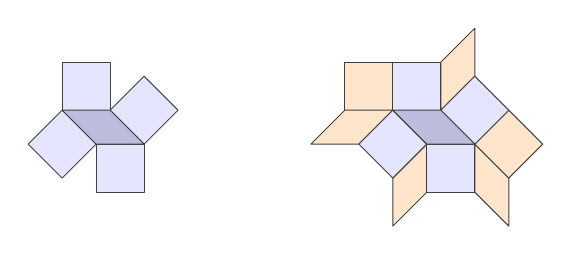
\begin{tikzpicture}[x=0.61cm,y=0.61cm,draw=black!75,line width=0.35pt,line join=round]
\def\drawcore{%
  \filldraw[fill=blue!10] (0,0) -- (1,0) -- (1,-1) -- (0,-1) -- cycle;
  \filldraw[fill=blue!10] (1,0) -- (0.2929,0.7071) -- (1,1.4142) -- (1.7071,0.7071) -- cycle;
  \filldraw[fill=blue!10] (0.2929,0.7071) -- (-0.7071,0.7071) -- (-0.7071,1.7071) -- (0.2929,1.7071) -- cycle;
  \filldraw[fill=blue!10] (-0.7071,0.7071) -- (0,0) -- (-0.7071,-0.7071) -- (-1.4142,0) -- cycle;
  \filldraw[fill=blue!32!gray!40] (0,0) -- (1,0) -- (0.2929,0.7071) -- (-0.7071,0.7071) -- cycle;
}
\drawcore
\begin{scope}[xshift=4.20cm]
  \filldraw[fill=orange!20] (0,0) -- (-0.7071,-0.7071) -- (-0.7071,-1.7071) -- (0,-1) -- cycle;
  \filldraw[fill=orange!20] (1,0) -- (1,-1) -- (1.7071,-1.7071) -- (1.7071,-0.7071) -- cycle;
  \filldraw[fill=orange!20] (1,0) -- (1.7071,-0.7071) -- (2.4142,0) -- (1.7071,0.7071) -- cycle;
  \filldraw[fill=orange!20] (0.2929,0.7071) -- (1,1.4142) -- (1,2.4142) -- (0.2929,1.7071) -- cycle;
  \filldraw[fill=orange!20] (-0.7071,0.7071) -- (-0.7071,1.7071) -- (-1.7071,1.7071) -- (-1.7071,0.7071) -- cycle;
  \filldraw[fill=orange!20] (-0.7071,0.7071) -- (-1.7071,0.7071) -- (-2.4142,0) -- (-1.4142,0) -- cycle;
\drawcore
\end{scope}
\end{tikzpicture}\par
{\small A $45^\circ$ central tile with its four edge-neighbors (left) and one completed first corona (right).}
\end{center}

\newpage
\section{A closed formula for the labeled first corona}
For $b\in\{k,\ell\}$ put $c=n-b$, $h=b-1$, and define
\begin{align}
 S_b&=N-b-\cc{N-b}{2},\nonumber\\
 M_b&=\cc{h+4}{5}+(2c+3)\cc{h+3}{4}
  +\big((c+1)(c+3)+S_b\big)\cc{h+2}{3} \nonumber\\[-2pt]
 &\hspace{12em}+\big((c+1)^2+S_b\big)\cc{h+1}{2},\label{eq:mark}\\
 P&=N^4+2N^2(S_k+S_\ell)+S_k^2+S_\ell^2.\label{eq:P}
\end{align}
A binomial coefficient with nonnegative upper argument smaller than the lower argument is zero. Quantities indexed by $k$ and $\ell$ occur with their displayed multiplicities also when $k=\ell$.
\begin{theorem}\label{th:main}
For every admissible pair,
\begin{equation}\label{eq:main}
 \boxed{\displaystyle A(n,k)=\frac{4^n P-2^{n+1}(M_k+M_\ell)}{16}+n-2.}
\end{equation}
\end{theorem}

\paragraph{Expanding the composition counts.}
Write $H(0)=1$ and $H(s)=2^{s-1}$ for $s>0$. These count unrestricted compositions, by choosing the breaks between successive units. Every legal gap is less than $2n$, since $s_i\le b_i+N-1$. In this range,
\[
 f_n(s)=H(s)-\one_{s\ge n}(s-n+2)2^{s-n-1}.
\]
Indeed, the series of the bounded compositions is $(1-x)/(1-2x+x^n)$. Through degree $2n-1$, this is $(1-x)/(1-2x)-x^n(1-x)/(1-2x)^2$. The subtraction at $s=n$ is exactly one.

Substitute the expansion in \eqref{eq:jeffery}. Choosing the $H$ term at all four vertices gives $4^n/16$ times the sum over cores of $2^{\#\{i:s_i=0\}}$. This sum is $P$. To see it, let $d=j_i-j_{i-1}$ and write
\[
 W_b(d)=\one_{d=b}-\one_{d>b}.
\]
The factor $1+W_b(d)$ gives weight two at equality, one below, and zero above. Two neighboring $W$ factors cannot both be nonzero, since consecutive jumps would total at least $k+\ell=n$ between labels whose difference is at most $n-2$. A single $W_b$ sums to $S_b$ over its two labels, by counting differences equal to $b$ or greater than $b$. Opposite edges use disjoint pairs of labels. Expansion over all four labels gives exactly \eqref{eq:P}.

Choosing two subtractions requires two gaps of size $n$ and two of size zero, by their total $2n$. The zero gaps cannot be adjacent by the jump argument. In an alternating pattern the labels take two levels, separated by $k$ or by $\ell$, according to the pattern. The lower level has $N-k$ or $N-\ell$ possible placements. Each contributes one, giving $(N-k)+(N-\ell)=n-2$. Three subtractions are impossible. It remains to evaluate the single subtractions.

\newpage
\paragraph{A single marked gap.}
Fix a vertex of type $b$ at which the subtraction is used. In cyclic order denote the two labels on its sides by $v,u$ and the next two by $w,z$. Then $v-u\ge c$. After extracting $2^{n-4}$, the contribution is $(v-u-c+2)$ times the product of $1+W$ on the other three edges. The total exponent follows from $\sum s_i=2n$, with each zero gap receiving its additional factor of two.

The three respective corrections are $W_c(w-u),W_b(z-w),W_c(v-z)$. The middle correction cannot coexist with either neighbor. Its sum over $w,z$ is $S_b$. The other two factors separate. Write $v=c+v'$ so $1\le u\le v'\le h=N-c$. Summing $W_c(w-u)$ over $w$ gives $u+1-h$, and summing $W_c(v-z)$ over $z$ gives $2-v'$. Including the constant terms, the remaining sum for this marked vertex becomes
\[
 \sum_{1\le u\le v'\le h}(v'-u+2)
       \big[(N+u+1-h)(N+2-v')+S_b\big].
\]
Set $i=u-1$, $j=v'-u$, $t=h-v'$. Then $i+j+t=h-1$, and the summand is $(j+2)((c+2+i)(c+2+t)+S_b)$. Its sum is the coefficient of $x^{h-1}$ in
\[
 \frac{(2-x)(c+2-(c+1)x)^2}{(1-x)^6}
       +S_b\frac{2-x}{(1-x)^4}.
\]
A coefficient with index $-1$ is zero. Replacing $2-x$ by $1+(1-x)$ and $c+2-(c+1)x$ by $1+(c+1)(1-x)$ gives \eqref{eq:mark}. Each of the two vertex types occurs twice, proving Theorem~\ref{th:main}. \hfill$\square$

\begin{theorem}\label{th:conseq}
Every fixed column of $A$ has least constant-coefficient recurrence order 13. For all $n\ge3$, every entry in row $n$ is $n-2$ modulo $2^{n-3}$. In column one, this modulus is sharp exactly when $n\equiv4,6\pmod8$.
\end{theorem}
\begin{proof}
With $k$ fixed, $S_k=-n^2/2+O_k(n)$ while $S_\ell$ is constant, so $P$ is a quartic with leading coefficient $1/4$. In $M_\ell$, $h=n-k-1$ varies and $c=k$ is fixed. Its leading term is $n^5/120$. The degree of $M_k$ is at most two. Formula \eqref{eq:main} thus contains three exponentials of bases $4,2,1$ times polynomials of exact degrees $4,5,1$. For $\lambda^n p(n)$ the operator $E-\lambda$ lowers the polynomial degree by one, and each $E-\mu$ with $\mu\ne\lambda$ preserves it. Applying the other factors to isolate a base proves minimality (equivalently the distinct exponential-polynomial spaces form a direct sum). This proves the stated order and also $A(n,k)\sim4^n n^4/64$.

The quotient $(A-(n-2))/2^{n-3}$ equals $2^{n-1}P-M_k-M_\ell$. In column one $M_1=0$ and \eqref{eq:mark} gives $M_{n-1}\equiv\binom{n+2}{5}+\binom{n+1}{4}\equiv\binom{n+1}{5}\pmod2$. In $(1+x)^{n+1}$ over $\mathbb F_2$, the coefficient of $x^5$ is one exactly when the $1$ and $4$ bits of $n+1$ are set, giving the two claimed classes. The exceptional row $n=2$ consists of $A(2,1)=1$.
\end{proof}

\newpage
\section{The four edge-neighbors and their symmetry classes}
Put $U=\binom{\ell-1}{2}$ and $V=\binom{k-1}{2}$. Write $C$ for the labeled core count (\oid{233330}) and $B$ for the core count up to isometry (\oid{233331}). Introduce
\[
 H_2=N^2-U-V,\qquad L_b=\floor{(n+b)/2},\qquad F_b=L_b^2-\cc{b-1}{2}.
\]
\begin{theorem}\label{th:core}
The labeled and symmetry-reduced core counts are
\begin{align*}
 C&=N^4-2N^2(U+V)+U^2+V^2,\\
 B&=\begin{cases}
 (C+H_2+F_k+F_\ell)/4,& n>2k,\\
 (C+H_2+2F_k+4N)/8,& n=2k .
 \end{cases}
\end{align*}
The fifth forward difference of every column of $C$ vanishes. For $B$, the reduced column generating function has denominator $(1-x)^5(1+x)^2$.
\end{theorem}
\begin{proof}
A jump of more than $b$ occurs in $\binom{N-b}{2}$ ordered pairs. Neighboring violations are impossible and opposite violations use disjoint labels. Inclusion-exclusion yields $C$. Its degree in $n$ for fixed $k$ is four, with leading coefficient $1/4$.

A nonsquare central tile has a half-turn and two diagonal reflections besides the identity. A half-turn fixes label tuples $(u,v,u,v)$ with $u-v\le k$ and $v-u\le\ell$, giving $H_2$. A reflection sending vertex $i$ to $t-i$ reverses the directed edges, so it sends $j_i$ to $n-j_i$ at edge $t-i-1$. For $t=0$ a fixed tuple is $(u,n-w,w,n-u)$. Its four gaps, in cyclic order, are
\[
 n+k-2u,\quad u+w-k,\quad n+k-2w,\quad u+w-k.
\]
There are $L_k^2$ pairs with $1\le u,w\le L_k$, of which $\binom{k-1}{2}$ fail $u+w\ge k$. This gives $F_k$. The other diagonal interchanges $k$ and $\ell$. On a square there are two more rotations (quarter-turns), each fixing the $N$ constant tuples. Each of the two additional reflections is through opposite edge midpoints. It fixes those two edge labels at $k=n/2$ and exchanges the other two complementary labels, giving $N$ choices. Burnside's lemma gives both formulas.

For fixed $k$, only $F_k$ has a parity-dependent term on $n>2k$, since $L_\ell=n-\lceil k/2\rceil$. Its alternating part has degree one and a nonzero linear coefficient from $L_k^2$. The ordinary polynomial part of $B$ has degree four. Changing the value at $n=2k$ adds a polynomial to the column generating function and preserves its poles.
\end{proof}

In particular $\sum_{n\ge2} B(n,1)x^n=x^2(1+4x+x^2)/((1-x)^5(1+x)^2)$. Indeed the two symmetry formulas agree at $(2,1)$, and multiplying the stated denominator by the series beginning $x^2(1+7x+21x^2+51x^3+102x^4+186x^5+310x^6+\cdots)$ gives that numerator. The proved recurrence determines subsequent coefficients. This identifies $B(n,1)$ with \oid{233329}$(n-2)$. Substitution at $n=2m$ gives $B(2m,1)=m(m+1)(2m^2-1)/2$, the value of \oid{076454}$(m)$. Indeed the uniquely represented values $tm+u(m+1)$ have $0\le t\le m$, $0\le u<m$, because any other representation changes $(t,u)$ by a multiple of $(m+1,-m)$. Summing over this rectangle gives the formula.

\newpage
\section{The filled first corona up to isometry}
Write $O(n,k)$ for the count of first coronas under the isometries preserving the central rhombus, as in the definition of \oid{233333}. Let $R$ count fixed patches under the half-turn, and $D_b$ those fixed by the diagonal through the two vertices whose gaps have type $b$.  Put
\begin{align*}
 R&=2^{n-2}(H_2+n-2)-(n-2),\\
 J_b&=\floor{b/2},\quad X_b=L_b^2-\cc{b-1}{2}+b-1,\quad
 Y_b=J_b(L_b-b+2)+\cc{J_b+1}{2},\\
 D_b&=2^{n-1-((n+b)\bmod 2)}X_b-2^{L_b+J_b-b}Y_b
              +\one_{2\mid b}-\one_{2\mid(n+b)} .
\end{align*}
\begin{theorem}\label{th:orbits}
If $T=A(n,k)+R+D_k+D_\ell$, the symmetry count is
\[
 O(n,k)=\begin{cases}
 T/4,&n>2k,\\
 \big(T+2N(2^{k-1}+2^{n-2})\big)/8,&n=2k .
 \end{cases}
\]
\end{theorem}
\begin{proof}
At a half-turn the two independent sectors have sizes $s$ and $n-s$. For $0<s<n$ their filling count is $2^{n-2}$. At either endpoint it is $2^{n-1}-1$. Of the $H_2$ fixed cores, $(N-k)+(N-\ell)=n-2$ give an endpoint, proving the formula for $R$.

A diagonal reflection reverses the compositions at its two fixed vertices and interchanges the other two compositions, reversing their order. Write $p_n(s)$ for the number of palindromic allowed compositions. For $0\le s<2n$,
\[
 p_n(s)=2^{\lfloor s/2\rfloor}
       -\one_{s\ge n}2^{\lfloor(s-n)/2\rfloor}.
\]
Unrestricted palindromes correspond to symmetric sets of breaks. Any part of size at least $n$ has to be the middle part. Its left half is an arbitrary composition of total at most $\lfloor(s-n)/2\rfloor$, which gives the subtracted count including the empty choice.

Use the fixed tuple in the core proof and replace $k$ by $b$. For $u,w\le L_b$, $u+w\ge b$, the number of fillings is
\[
 p_n(n+b-2u)\,p_n(n+b-2w)\,f_n(u+w-b).
\]
Write $L=L_b$, $J=J_b$, $a_u=2^L-\one_{u\le J}2^J$. The first palindrome factor is $2^{-u}a_u$. The free sector size $s=u+w-b$ is at most $n$. Multiplying the unrestricted positive-size formula $2^{s-1}$ into the palindrome factors gives $2^{-b-1}a_u a_w$. Give $s=0$ twice this weight. If $s=n$, subtract one forbidden single part. That endpoint exists just when $n+b$ is even and has $u=w=L$, with both palindromes empty.

The weight $\one_{u+w\ge b}+\one_{u+w=b}$ sums on the $L\times L$ box to $X_b$. On the first $J$ rows it sums to $Y_b$, since row $u$ loses $b-u-1$ entries and gains one equality. On the $J\times J$ box it sums to $2\one_{2\mid b}$. Expanding $a_u a_w$ now gives $D_b$. For a square each quarter-turn fixes $N f_n(k)=N2^{k-1}$ fillings. A reflection through edge midpoints leaves two free sectors of sizes $u, n-u$, $1\le u\le N$, one pair per fixed core. It fixes $N2^{n-2}$ fillings. Averaging proves the theorem.
\end{proof}

\newpage
\section{Least recurrence after identifying isometries}
\begin{theorem}\label{th:twenty}
For every fixed $k$, the least eventual characteristic polynomial of $O(n,k)$ is
\[
 \boxed{(E-4)^5(E-2)^6(E+2)^3(E^2-2)^3.}
\]
It has order 20 and holds from $n=2k+1$. At $k=1$ it holds from $n=2$. For $k\ge2$ a recurrence valid starting at $n=2k$ has least polynomial $E$ times the displayed polynomial.
\end{theorem}
\begin{proof}
Extend the nonsquare expression $O_*=T/4$ to $n=2k$. In $4O_*$ the residual $n-2$ in $A$ cancels the residual $-(n-2)$ in $R$. The indicator terms from $D_k,D_\ell$ also cancel, since $n+k$ has the parity of $\ell$ and $n+\ell$ that of $k$. The $4^n$ polynomial is quartic. The contributions at base $2$ from $A$ and $R$ have a common parity-independent polynomial of degree five. The remaining terms of size $2^n$ have a polynomial coefficient on each parity, of degree at most two, from $X_k$ and $X_\ell$.

To detect a $(-2)^n$ term of degree two, divide those two $X$ terms by $2^n$. The leading coefficients in $X_k,X_\ell$ are respectively $1/4,1/2$, since $L_k=n/2+O_k(1)$ and $L_\ell=n+O_k(1)$. The resulting coefficients of $n^2$, after the parity factors from $D_b$, are
\[
\begin{array}{c|cc}
 & n\text{ even} & n\text{ odd}\\ \hline
 k\text{ even} & 3/8 & 5/16\\
 k\text{ odd}  & 3/16 & 1/4 .
\end{array}
\]
Each row has unequal entries. Splitting a pair of parity polynomials into its average and its alternating part proves that the degree at base $-2$ is exactly two.

Finally $Y_k$ has degree at most one on each parity, and $Y_\ell$ has leading coefficient $1/8$ at degree two. In $D_\ell$ the factor $2^{L_\ell+J_\ell-\ell}/(\sqrt2)^n$ equals $2^{-(k\bmod2)}$ on even $n$ and $1/\sqrt2$ on odd $n$. These positive numbers are unequal. Both their average and their difference are nonzero. Thus the two bases $\sqrt2,-\sqrt2$ each have degree two. The distinct-base argument in Theorem~\ref{th:conseq} proves the least polynomial.

At $n=2k$, $O_*$ counts orbits under the four-element subgroup. For $k=1$ there is one patch. For $k\ge2$, take the legal core $(k+1,k,k,k)$ and fill each sector with ones. A quarter-turn takes the $+1$ perturbation to a neighboring edge. The subgroup moves it only to its opposite edge by rotation, or changes it to a $-1$ perturbation by reflection. Hence the full square group strictly merges subgroup orbits. The difference between $O$ and $O_*$ has support just at the first index. It is killed by $E$ and the displayed polynomial has nonzero constant term. This proves the final assertion.
\end{proof}

For $(n,k)=(4,1)$, the identity, half-turn and two reflections fix $1452$, $38$, $16$ and $34$ patches. Their average is $385$. Four singleton orbits, 38 pairs and 343 orbits of size four account for every one of the $1452$ patches. The corresponding square counts give $247$, in agreement with the entry. Thus the first three rows under the stated symmetry convention are $(1)$, $(28)$ and $(385,247)$.

\newpage
\section{Arithmetic progressions and checks}

Jeffery's companion array \oid{235804} has entries $T(n,j)=n-2+j2^{n-3}$, for $n\ge3$, $j\ge0$. Theorem~\ref{th:conseq} puts the corona counts in the indicated residue class. They occur in the nonnegative progression as well. For example, each of the $N=n-1$ constant label quadruples has strictly positive gaps and admits at least one filling, so $A(n,k)\ge n-1$.

Summing the arithmetic progression in $j$ and its two summands in $n$ gives the proposed generating functions.
\begin{align*}
 \sum_{j\ge0}T(n,j)x^j
   &=\frac{(n-2)+(2^{n-3}-(n-2))x}{(1-x)^2},\\
 \sum_{i\ge0}T(i+3,j)x^i
   &=\frac{1}{(1-x)^2}+\frac{j}{1-2x}
     =\frac{j+1-2(j+1)x+jx^2}{(1-2x)(1-x)^2}.
\end{align*}
The sum on antidiagonal $i+j=t$, starting at $t=0$, is
\[
 \sum_{i=0}^t\big(i+1+(t-i)2^i\big)
    =2^{t+1}-1+\cc{t+1}{2}=\text{\oid{132925}}(t+1).
\]
Here $\sum_{i=0}^t(t-i)2^i=2^{t+1}-t-2$ by a finite geometric sum.

\paragraph{Reproducibility.}
The file \texttt{verify.py} directly enumerates Jeffery's four-label sums at every admissible pair through $n=16$ and complete word orbits through $n=6$. It also evaluates the unsimplified symmetry sums through $n=52$ and checks both recurrence formulas in twenty fixed columns. Independently enumerated Hankel matrices in the first three columns have nonzero determinants at the two claimed orders. The optional OEIS comparison reproduces the published lists and identifies the single discrepancy discussed above.

The separate program \texttt{geometry\_n4.py} constructs polygons directly in $\mathbb Z[e^{\pi i/4}]$. It enumerates the allowable rays around each central vertex, checks pairwise tile compatibility, then compares the exact vertex sets under the isometries of the marked central tile. Its two orbit counts are 385 and 247. The file \texttt{Certificate.lean} checks the four and eight fixed-set sizes by enumerating the ordered sector fillings and verifies both Burnside averages in the Lean 4.19 kernel. The all-parameter proofs are given in Sections 2--5.

\begin{thebibliography}{9}
\bibitem{jeffery}
L. Edson Jeffery, \emph{On the number of coronas of a fixed rhombus with characteristics of $n$-fold symmetry in $\mathbb R^2$}, author manuscript attached to OEIS \oid{233332}, especially pp.~2--4.
\href{https://oeis.org/A233332/a233332_5.pdf}{Full text}.
\bibitem{oeis}
OEIS Foundation Inc., \emph{The On-Line Encyclopedia of Integer Sequences}.
L. Edson Jeffery's entries \oid{233329}, \oid{233330}, \oid{233331}, \oid{233332}, \oid{233333} and \oid{235804} record the conjectures, data and definitions. The companion sequences are Floor van Lamoen's \oid{076454} and Gary W. Adamson's \oid{132925}.
\href{https://github.com/oeis/oeisdata/tree/976b0c73e00453b1c1e6f16d83108cb9bb744c3b}{Version used for data checks}.
\end{thebibliography}
\end{document}
